\documentclass[11pt,a4paper]{article}
\usepackage[utf8]{inputenc}
\usepackage[margin=2.2cm]{geometry}
\usepackage{tikz}
\usetikzlibrary{shapes.geometric,arrows.meta,positioning,calc,fit,backgrounds,decorations.pathreplacing,patterns}
\usepackage{xcolor}
\usepackage{enumitem}
\usepackage{amsmath,amssymb}
\usepackage{booktabs}
\usepackage{hyperref}
\usepackage{array}
\usepackage{tabularx}
\usepackage{float}

\definecolor{teachcol}{RGB}{41,128,185}
\definecolor{studcol}{RGB}{39,174,96}
\definecolor{clustcol}{RGB}{142,68,173}
\definecolor{structcol}{RGB}{211,84,0}
\definecolor{pilecol}{RGB}{44,62,80}
\definecolor{slotcol}{RGB}{46,204,113}
\definecolor{physloss}{RGB}{231,76,60}
\definecolor{dataloss}{RGB}{52,152,219}
\definecolor{timcol}{RGB}{230,126,34}

\title{\textbf{The $\Psi$-NN Method (Liu et al., 2025)}\\[0.3cm]
\large Detailed Explanation of the Paper and Its Application\\[0.1cm]
to Predicting Pile Stiffness Degradation\\[0.1cm]
in the Post-Typhoon OWT Project}
\author{}
\date{}

\begin{document}
\maketitle
\tableofcontents
\newpage

%% ============================================================
%%  PART A: EXPLAINING THE PAPER
%% ============================================================

\part{The $\Psi$-NN Paper Explained}

\section{What Is This Paper About?}

The paper is titled:

\begin{quote}
\textit{``Automatic Network Structure Discovery of Physics-Informed Neural Networks via Knowledge Distillation''}\\
--- Ziti Liu, Yang Liu, Xunshi Yan, Wen Liu, Han Nie, Shuaiqi Guo, Chen-an Zhang\\
Published in \textbf{Nature Communications} (2025), DOI: 10.1038/s41467-025-64624-3
\end{quote}

In simple words, the paper proposes a method called $\Psi$-NN that can \textbf{automatically discover the best internal structure of a neural network} so that the network respects the physics of the problem it is solving.

\subsection{The Problem It Solves}

When we use neural networks to solve physics problems (like differential equations), we face a dilemma:

\begin{enumerate}[nosep]
    \item \textbf{Standard neural networks} (fully connected, generic) work on any problem, but they are slow to train, need lots of data, and do not guarantee that the solution obeys physical laws (like symmetry or energy conservation).
    \item \textbf{Manually structured networks} (where a human designs the architecture to match the physics) are faster and more accurate, but they require \textit{expert knowledge} for every new problem, and their design does not generalize.
\end{enumerate}

$\Psi$-NN solves this by saying: \textit{``Let the training process itself discover which structure the network should have, automatically, by looking at the data and the physical equations together.''}

\subsection{Why Is This Hard?}

Physics-informed neural networks (PINNs) already embed physics by adding PDE residuals to the loss function. But PINNs do not change the \textit{internal wiring} of the network. All neurons remain fully connected. The physics is only applied as a penalty, not as a structural constraint.

If you try to add structural penalties (like regularization to remove unnecessary connections), you run into a conflict:

\begin{itemize}[nosep]
    \item The physics loss says: ``make the PDE residual small.''
    \item The regularization loss says: ``make the weights small or zero.''
    \item These two objectives pull the optimizer in opposite directions, and the network fails to converge properly.
\end{itemize}

This is the core insight of the paper: \textbf{you cannot do both at the same time in a single network}.

\section{The Three-Stage $\Psi$-NN Method}

The solution is a three-stage pipeline:

\begin{center}
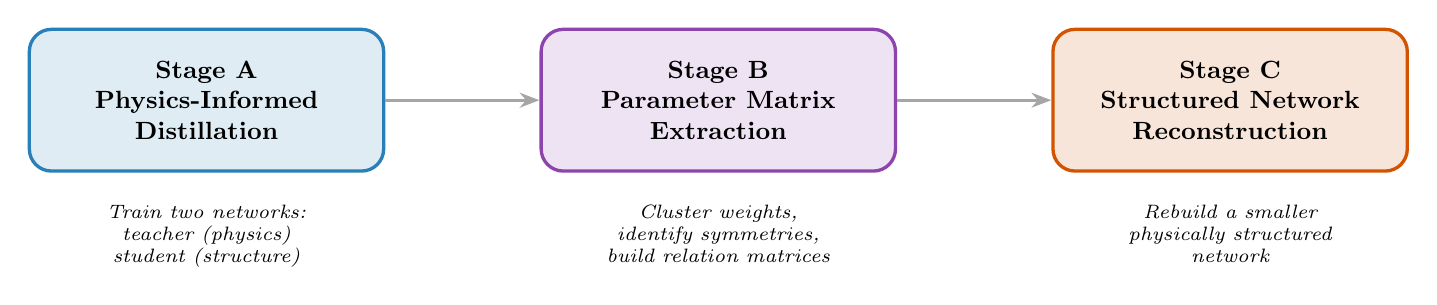
\begin{tikzpicture}[
    >={Stealth[length=2.5mm]},
    stage/.style={rectangle, rounded corners=8pt, minimum width=4.5cm, minimum height=1.8cm, align=center, font=\small\bfseries, draw, line width=1.2pt},
    arrow/.style={->, thick, gray!70, line width=1.2pt},
    note/.style={font=\scriptsize\itshape, align=center, text width=4.2cm},
]
\node[stage, fill=teachcol!15, draw=teachcol] (A) at (0,0) {Stage A\\Physics-Informed\\Distillation};
\node[stage, fill=clustcol!15, draw=clustcol] (B) at (6.5,0) {Stage B\\Parameter Matrix\\Extraction};
\node[stage, fill=structcol!15, draw=structcol] (C) at (13,0) {Stage C\\Structured Network\\Reconstruction};

\draw[arrow] (A) -- (B);
\draw[arrow] (B) -- (C);

\node[note, below=8pt of A] {Train two networks:\\teacher (physics)\\student (structure)};
\node[note, below=8pt of B] {Cluster weights,\\identify symmetries,\\build relation matrices};
\node[note, below=8pt of C] {Rebuild a smaller\\physically structured\\network};
\end{tikzpicture}
\end{center}

\subsection{Stage A: Physics-Informed Distillation}

This stage uses \textbf{two separate networks} trained in sequence:

\subsubsection*{The Teacher Network}

The teacher is a standard PINN. It is trained with:
$$
\mathcal{L}_{\text{teacher}} = \mathcal{L}_{\text{data}} + \lambda_{\text{PDE}} \cdot \mathcal{L}_{\text{PDE}}
$$

where:
\begin{itemize}[nosep]
    \item $\mathcal{L}_{\text{data}}$ measures how well the network fits the available data points.
    \item $\mathcal{L}_{\text{PDE}}$ measures how well the network satisfies the governing partial differential equation (PDE).
\end{itemize}

The teacher learns to solve the physics problem accurately, but its weights are messy --- there is no visible structure in them.

\subsubsection*{The Student Network}

After the teacher converges, the student is trained to \textbf{imitate the teacher's output} while also being pushed to have a clean, structured weight matrix:

$$
\mathcal{L}_{\text{student}} = \mathcal{L}_{\text{distill}} + \mu \cdot \mathcal{L}_{\text{reg}}
$$

where:
\begin{itemize}[nosep]
    \item $\mathcal{L}_{\text{distill}}$ is the distillation loss: the student must match the teacher's predictions.
    \item $\mathcal{L}_{\text{reg}}$ is a parameter regularization term (e.g., L1 or L2) that encourages simple, sparse, or symmetric weight patterns.
\end{itemize}

The key idea: the student \textbf{does not see the PDE loss}. It only learns from the teacher. This way, the regularization term does not conflict with the physics loss, because they live in different networks.

\begin{center}
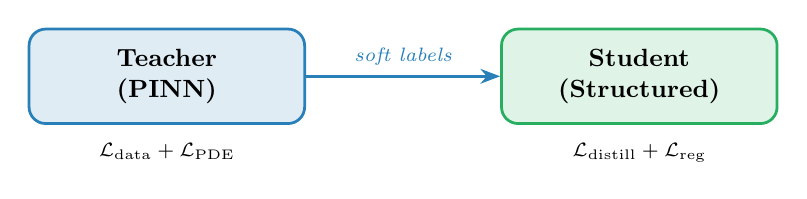
\begin{tikzpicture}[
    >={Stealth[length=2.5mm]},
    block/.style={rectangle, rounded corners=6pt, minimum width=3.5cm, minimum height=1.2cm, align=center, font=\small\bfseries, draw, line width=1pt},
    arrow/.style={->, thick, line width=1pt},
]
\node[block, fill=teachcol!15, draw=teachcol] (teacher) at (0,0) {Teacher\\(PINN)};
\node[block, fill=studcol!15, draw=studcol] (student) at (6,0) {Student\\(Structured)};
\node[font=\scriptsize, below=3pt of teacher] {$\mathcal{L}_{\text{data}} + \mathcal{L}_{\text{PDE}}$};
\node[font=\scriptsize, below=3pt of student] {$\mathcal{L}_{\text{distill}} + \mathcal{L}_{\text{reg}}$};

\draw[arrow, teachcol] (teacher) -- node[above, font=\scriptsize\itshape] {soft labels} (student);
\end{tikzpicture}
\end{center}

\subsection{Stage B: Parameter Matrix Extraction}

Once the student is trained, its weight matrices contain patterns --- for example:
\begin{itemize}[nosep]
    \item Some weights are almost identical $\Rightarrow$ they can be replaced by a single shared value.
    \item Some weights are the negative of others $\Rightarrow$ they encode a symmetry ($u(x) = -u(-x)$, etc.).
    \item Some biases are nearly zero $\Rightarrow$ they can be removed.
\end{itemize}

The extraction process is:
\begin{enumerate}[nosep]
    \item \textbf{Clustering}: Apply a clustering algorithm (like k-means) to the weight values in each layer. Weights with similar values are assigned to the same cluster center.
    \item \textbf{Relation matrix construction}: For each layer, a relation matrix $\mathbf{R}_l$ is built. This matrix describes rules like:
    \begin{itemize}[nosep]
        \item ``Row 2 = Row 1'' (reuse)
        \item ``Row 3 = $-$Row 1'' (sign reversal)
        \item ``Row 4 = Swap of Row 2'' (permutation)
    \end{itemize}
\end{enumerate}

These relation matrices are a compact symbolic description of the hidden structure.

\subsection{Stage C: Structured Network Reconstruction}

Using the relation matrices, a new network is built from scratch. This network is smaller, faster, and \textbf{has the discovered structure hardwired into its architecture}:

\begin{itemize}[nosep]
    \item Shared weights reduce the number of trainable parameters.
    \item Sign reversals and permutations enforce symmetries at every forward pass.
    \item The network can be retrained on new data or new parameter values while keeping its discovered structure.
\end{itemize}

The result is a physics-structured neural network that:
\begin{enumerate}[nosep]
    \item Converges faster (50\% fewer iterations on Laplace equation).
    \item Is more accurate (95\% lower L2 error on Laplace equation).
    \item Generalizes to different parameter values without retraining the structure.
    \item Can transfer its structure to entirely different problems with similar physics.
\end{enumerate}

\section{Detailed Results from the Paper}

The paper tests $\Psi$-NN on four problems:

\subsection{Laplace Equation}

$$\nabla^2 u = 0$$

The Laplace equation has clear spatial symmetry. $\Psi$-NN discovered this symmetry automatically:

\begin{itemize}[nosep]
    \item The extracted relation matrix showed that the two hidden neurons were related by the transformation $u_a(x_1, x_2) = u_b(x_1, -x_2)$.
    \item This is the exact symmetry of the boundary conditions.
    \item Result: 95\% lower error than standard PINN, 50\% fewer training iterations.
\end{itemize}

\subsection{Burgers Equation}

$$u_t + u \cdot u_x = \nu \cdot u_{xx}$$

This is a nonlinear PDE with a shock wave. The paper tested both the forward problem (predict the solution) and the inverse problem (find the unknown viscosity $\nu$):

\begin{itemize}[nosep]
    \item $\Psi$-NN discovered an anti-symmetry structure around the shock.
    \item Error was uniformly reduced on both sides of the shock, unlike PINN-post which only symmetrized the error but did not reduce it.
    \item For the inverse problem, $\Psi$-NN estimated $\nu$ closest to the true value across three different viscosity settings.
    \item The discovered structure transferred across different $\nu$ values without modification.
\end{itemize}

\subsection{Poisson Equation}

$$\nabla^2 u = f(x_1, x_2)$$

with a four-frequency source term. This is a harder problem because the solution has complex permutation symmetry:

\begin{itemize}[nosep]
    \item $\Psi$-NN extracted a low-frequency structure first, then adapted it by sign adjustment to capture the high-frequency symmetry.
    \item The extracted weight matrices showed a clean block structure matching the $\mathbb{Z}_2 \times \mathbb{Z}_2$ equivariant group.
\end{itemize}

\subsection{2D Cylinder Flow (Navier--Stokes)}

$$\rho(\mathbf{u} \cdot \nabla)\mathbf{u} + \nabla p - \mu \nabla^2 \mathbf{u} = 0$$

This is the most complex test --- a real fluid mechanics problem with two outputs ($u$, $v$) that have opposite symmetries:

\begin{itemize}[nosep]
    \item $u$ (horizontal velocity) is symmetric about the centerline.
    \item $v$ (vertical velocity) is anti-symmetric about the centerline.
    \item $\Psi$-NN successfully applied the Laplace-derived structure to $u$ and the Burgers-derived structure to $v$.
    \item This demonstrated \textbf{cross-problem structural transfer}: structures found in simple PDEs can be reused in complex problems.
\end{itemize}

\subsection{Summary of Paper Results}

\begin{table}[H]
\centering
\begin{tabular}{@{}lccc@{}}
\toprule
\textbf{Test Case} & \textbf{PINN (L2)} & \textbf{PINN-post (L2)} & \textbf{$\Psi$-NN (L2)} \\
\midrule
Laplace (symmetry) & $2.26 \times 10^{-2}$ & $7.64 \times 10^{-3}$ & $\mathbf{1.03 \times 10^{-3}}$ \\
Burgers (shock) & $2.03 \times 10^{-1}$ & $1.14 \times 10^{-1}$ & $\mathbf{6.82 \times 10^{-2}}$ \\
Poisson (high-freq) & $4.20 \times 10^{-2}$ & $3.59 \times 10^{-2}$ & $\mathbf{1.62 \times 10^{-2}}$ \\
\bottomrule
\end{tabular}
\caption{Full-field L2 errors from the paper. Lower is better. $\Psi$-NN is consistently the best.}
\end{table}

\section{What the Paper Does NOT Do}

It is important to understand the boundaries of this paper:

\begin{itemize}[nosep]
    \item It works on problems where the PDE is known (at least partially).
    \item It targets \textbf{symmetry-type} structural features (sign reversal, permutation, reuse).
    \item It does not address time-series sequential prediction (like stiffness degradation over load steps).
    \item It does not include a recurrent or transformer-based decoder.
    \item It does not directly handle thermodynamic constraints (energy conservation, dissipation).
\end{itemize}

These limitations define exactly where the adaptation to our pile degradation project becomes interesting and non-trivial.

%% ============================================================
%%  PART B: THE POST-TYPHOON OWT PROJECT
%% ============================================================

\part{The Post-Typhoon OWT Project}

\section{What Is the Post-Typhoon Project About?}

The Post-Typhoon project (Guangdong Provincial Natural Science Fund proposal) aims to:

\begin{quote}
\textit{Predict how the natural frequency ($f_0^{\text{OWT}}$) of an offshore wind turbine (OWT) supported by a monopile changes after a typhoon hits.}
\end{quote}

\subsection{Why Does This Matter?}

Offshore wind turbines are designed with a ``soft-stiff'' approach: their natural frequency $f_0$ sits safely between the rotor frequency ($f_{1P}$) and the blade-passing frequency ($f_{3P}$):

$$f_{1P} < f_0^{\text{OWT}} < f_{3P}$$

When a typhoon applies extreme cyclic loads, the soil around the monopile weakens (stiffness degradation). This reduces the foundation stiffness ($K_L$, $K_R$, $K_{LR}$), which in turn lowers $f_0^{\text{OWT}}$. Even a 5--10\% shift can push $f_0$ into resonance with $f_{1P}$ or $f_{3P}$, amplifying vibrations by 150--300\% and potentially causing collapse.

\subsection{The Correlation Chain}

The project targets a three-step causal chain:

\begin{center}
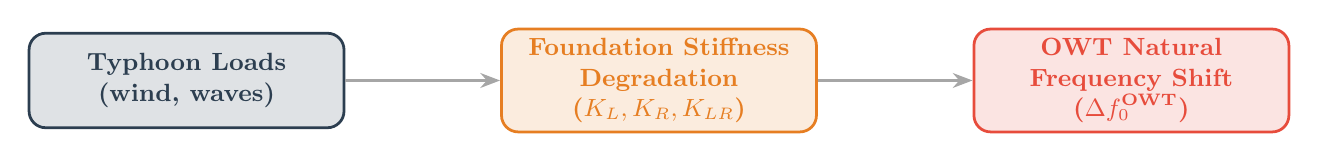
\begin{tikzpicture}[
    >={Stealth[length=2.5mm]},
    block/.style={rectangle, rounded corners=6pt, minimum width=4cm, minimum height=1.2cm, align=center, font=\small\bfseries, draw, line width=1pt},
    arrow/.style={->, thick, gray!70, line width=1.2pt},
]
\node[block, fill=pilecol!15, draw=pilecol, text=pilecol] (A) at (0,0) {Typhoon Loads\\(wind, waves)};
\node[block, fill=timcol!15, draw=timcol, text=timcol] (B) at (6,0) {Foundation Stiffness\\Degradation\\($K_L, K_R, K_{LR}$)};
\node[block, fill=physloss!15, draw=physloss, text=physloss] (C) at (12,0) {OWT Natural\\Frequency Shift\\($\Delta f_0^{\text{OWT}}$)};

\draw[arrow] (A) -- (B);
\draw[arrow] (B) -- (C);
\end{tikzpicture}
\end{center}

Currently, predicting this chain requires:
\begin{enumerate}[nosep]
    \item A high-fidelity FEM simulation of the soil-pile system (20--32 hours per scenario).
    \item A separate structural eigenvalue analysis to compute $f_0$.
\end{enumerate}

The project proposes replacing this two-stage workflow with a \textbf{single physics-informed transformer} that predicts $f_0^{\text{OWT}}$ shifts in near real-time.

\subsection{Key Architecture Elements Proposed}

The Post-Typhoon project proposes:

\begin{enumerate}[nosep]
    \item \textbf{A slot-attention self-calibration module}: 21 learned slots where:
    \begin{itemize}[nosep]
        \item Slot 1 learns the initial 3DOF stiffness matrix $H_0^{ij}$.
        \item Slots 2--21 each learn a plastic stiffness drop matrix $H_n^{ij}$ with a sigmoid activation gate $w_n(t)$.
    \end{itemize}
    \item \textbf{Physics-informed losses}: Laws of Thermodynamics (LoT1 = energy conservation via frequency consistency, LoT2 = non-negative dissipation via monotonic stiffness drops).
    \item \textbf{A full encoder-decoder transformer}: that maps typhoon loads $\rightarrow$ stiffness evolution $\rightarrow$ $f_0^{\text{OWT}}$ shifts.
    \item \textbf{XAI via attention mapping}: to open the black box and verify that the AI learned physically meaningful correlations.
\end{enumerate}

The foundation stiffness degradation is modeled via the TIM (Thermodynamic Inertial Macroelement):

$$H^{ij}(t) = H_0^{ij} - \sum_{n=1}^{20} w_n(t) \cdot H_n^{ij}$$

This is a core equation: stiffness at time $t$ equals the initial stiffness minus the sum of activated plastic drops.

%% ============================================================
%%  PART C: HOW PSI-NN CAN BE APPLIED
%% ============================================================

\part{Applying $\Psi$-NN to the Pile Degradation Project (M5)}

\section{The Starting Point: What M5 Already Does}

The M5 model is a Slot-Attention Transformer that was trained to predict a \textbf{21-step pile stiffness degradation sequence} ($K_L$, $K_R$, $K_{LR}$) from 8 input parameters (PI, $G_{\max}$, $\nu$, $D_p$, $T_p$, $L_p$, $I_p$, $D_p/L_p$).

Its architecture uses:
\begin{itemize}[nosep]
    \item \textbf{21 learnable slot vectors} of dimension 64. Slot 1 is assigned to predict the initial absolute stiffness values. Slots 2--21 are used to generate the 20 sequential degradation steps.
    \item \textbf{2-layer LSTM decoder} that builds predicted stiffness values step by step.
    \item \textbf{Physics constraint}: drops for $K_L$ and $K_R$ are forced to be non-positive by computing $-|\hat{d}|$.
    \item \textbf{Composite loss}: Huber loss on the full sequence + $3\times$ MSE on the first state + Huber loss on step-to-step differences (shape loss).
\end{itemize}

After training on 815 scenarios (out of 1019) for 928 epochs, M5 achieves:
\begin{itemize}[nosep]
    \item Overall $R^2 = 0.9913$
    \item $K_L$: $R^2 = 0.9907$, $K_R$: $R^2 = 0.9838$, $K_{LR}$: $R^2 = 0.9882$
\end{itemize}

M5 is already a strong model. The question $\Psi$-NN raises is: \textbf{can we look inside the trained model and understand \textit{why} it works so well?} And once we understand the internal structure it discovered, can we hardwire that structure into a rebuilt, lighter model?

\section{The Core Idea: M5 as the $\Psi$-NN Teacher}

In the $\Psi$-NN framework, the ``teacher'' is any network that has already been trained to solve the problem well, without restrictions on its internal structure. The teacher's job is done --- it has learned to be accurate.

\textbf{M5 is already a perfect teacher.} It was trained with:
\begin{itemize}[nosep]
    \item Data loss (Huber sequence loss) --- equivalent to $\mathcal{L}_{\text{data}}$.
    \item Physics constraint ($-|\hat{d}|$ for monotonic drops) --- equivalent to $\mathcal{L}_{\text{PDE}}$.
    \item Shape loss (step-to-step consistency) --- a structural regularity term.
\end{itemize}

We do not need to add any extra losses or change M5 at all. The trained M5 model, with its saved weights in \texttt{pile\_model.pth}, is the teacher. We feed it 1019 scenarios, record its 21 slot vectors and cross-attention patterns, and then apply the $\Psi$-NN structure discovery pipeline to those weights.

The three-stage $\Psi$-NN pipeline applied to M5:

\begin{center}
\resizebox{\textwidth}{!}{%
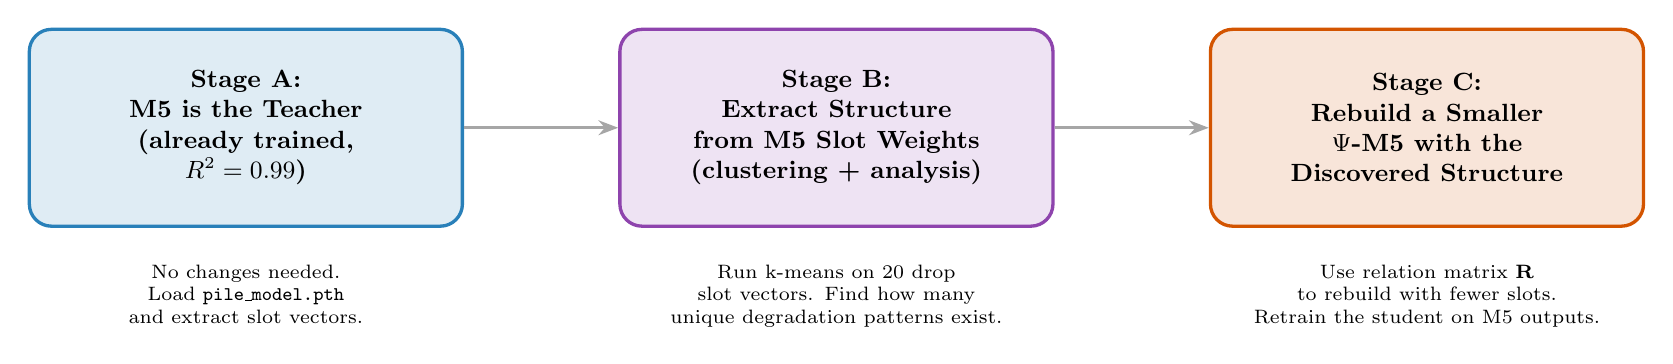
\begin{tikzpicture}[
    >={Stealth[length=2.5mm]},
    stage/.style={rectangle, rounded corners=8pt, minimum width=5.5cm, minimum height=2.5cm, align=center, font=\small\bfseries, draw, line width=1.2pt},
    arrow/.style={->, thick, gray!70, line width=1.2pt},
    note/.style={font=\scriptsize, align=center, text width=5cm},
]
\node[stage, fill=teachcol!15, draw=teachcol] (P1) at (0,0) {Stage A:\\M5 is the Teacher\\(already trained,\\$R^2 = 0.99$)};
\node[stage, fill=clustcol!15, draw=clustcol] (P2) at (7.5,0) {Stage B:\\Extract Structure\\from M5 Slot Weights\\(clustering + analysis)};
\node[stage, fill=structcol!15, draw=structcol] (P3) at (15,0) {Stage C:\\Rebuild a Smaller\\$\Psi$-M5 with the\\Discovered Structure};

\draw[arrow] (P1) -- (P2);
\draw[arrow] (P2) -- (P3);

\node[note, below=10pt of P1] {No changes needed.\\Load \texttt{pile\_model.pth}\\and extract slot vectors.};
\node[note, below=10pt of P2] {Run k-means on 20 drop\\slot vectors. Find how many\\unique degradation patterns exist.};
\node[note, below=10pt of P3] {Use relation matrix $\mathbf{R}$\\to rebuild with fewer slots.\\Retrain the student on M5 outputs.};
\end{tikzpicture}
}%
\end{center}

\section{Stage A: The Teacher (M5 as-is)}

No action is required here. The trained M5 model already contains a set of 21 learned slot vectors:

$$
\mathbf{S} = [\mathbf{s}_1,\; \mathbf{s}_2,\; \ldots,\; \mathbf{s}_{21}] \in \mathbb{R}^{21 \times 64}
$$

where each $\mathbf{s}_n$ is a 64-dimensional vector that M5 trained to specialize for one part of the degradation problem.

We also have:
\begin{itemize}[nosep]
    \item The cross-attention weight matrices: which input features each slot attends to.
    \item The LSTM hidden trajectories: how the decoder used slot information over 20 steps.
    \item The drop projection outputs: what 3-valued drop vector each decoder step produced.
\end{itemize}

All of this is extractable by running M5 in inference mode with the existing \texttt{pile\_model.pth} file.

\section{Stage B: Structure Discovery from M5 Slot Weights}

This is the heart of the $\Psi$-NN idea applied to M5. We extract and analyze the 20 drop-slot vectors $\mathbf{s}_2, \ldots, \mathbf{s}_{21}$.

\subsection*{Step B.1 --- Visualize the slot norms}

Compute $\|\mathbf{s}_n\|$ for $n = 2, \ldots, 21$. If the norms decrease with $n$, it means the model learned large early drops and small late drops --- which is physically expected for stiffness degradation. If the norms are roughly equal, it means all slots contribute equally.

\subsection*{Step B.2 --- Compute pairwise distances}

Compute the pairwise cosine similarity between all 20 drop slots:

$$
\text{sim}(i, j) = \frac{\mathbf{s}_i \cdot \mathbf{s}_j}{\|\mathbf{s}_i\| \cdot \|\mathbf{s}_j\|}
$$

If two slots are nearly identical ($\text{sim} \approx 1$), they encode the same degradation pattern and one can be removed. If two slots are nearly opposite ($\text{sim} \approx -1$), they encode a sign-reversal symmetry that can be expressed by a single slot with a sign rule.

\subsection*{Step B.3 --- Apply k-means clustering}

Apply k-means to the 20 drop-slot vectors for $k = 2, 3, \ldots, 10$. Use the \textbf{elbow method} (inertia curve) and \textbf{silhouette score} to find the natural number of independent slot groups $k^*$.

For example, if $k^* = 4$, then of the 20 drop slots, only 4 are truly unique degradation patterns. The remaining 16 are variations (scaled, sign-reversed, or near-duplicate copies) of those 4.

\subsection*{Step B.4 --- Build the relation matrix $\mathbf{R}$}

Once the $k^*$ cluster centers are identified, build a relation matrix $\mathbf{R}$ that describes how each of the 20 slots can be expressed using the $k^*$ unique prototypes:

\begin{itemize}[nosep]
    \item ``$\mathbf{s}_5 \approx \mathbf{s}_2$'' $\Rightarrow$ reuse rule: $\mathbf{s}_5 = \mathbf{s}_2$
    \item ``$\mathbf{s}_8 \approx -\mathbf{s}_3$'' $\Rightarrow$ sign-reversal rule: $\mathbf{s}_8 = -\mathbf{s}_3$
    \item ``$\mathbf{s}_{14} \approx 0.6 \cdot \mathbf{s}_2$'' $\Rightarrow$ scaling rule: $\mathbf{s}_{14} = 0.6 \cdot \mathbf{s}_2$
\end{itemize}

This relation matrix is a symbolic description of the hidden physics structure M5 discovered during training.

\subsection*{Step B.5 --- Check attention patterns}

In M5's cross-attention layers, each slot attends to the input embedding. Visualize the attention weights as a heatmap: rows = slots, columns = the 8 input features. Patterns to look for:

\begin{itemize}[nosep]
    \item Does Slot 1 (initial stiffness) attend most to $G_{\max}$ and $D_p$? This would make physical sense because initial stiffness depends on shear modulus and pile geometry.
    \item Do all drop slots share a similar attention pattern? If yes, they may not need separate slot vectors --- one representative is enough.
    \item Are there input features that no slot attends to? Those features may be irrelevant and could be removed.
\end{itemize}

\section{Stage C: Rebuild the $\Psi$-M5 Student}

Once the relation matrix $\mathbf{R}$ is known, build a new model called \textbf{$\Psi$-M5}:

\begin{itemize}[nosep]
    \item Instead of 21 freely learned slot vectors, $\Psi$-M5 has only $k^* + 1$ trainable slot vectors (1 for initial + $k^*$ unique drop prototypes).
    \item The full set of 21 slot vectors is reconstructed at each forward pass by applying $\mathbf{R}$: slot $n$ is computed as a fixed linear combination of the $k^*$ prototype slots.
    \item The rest of the architecture (LSTM, cross-attention, drop projection) remains unchanged.
\end{itemize}

The student ($\Psi$-M5) is then trained using the \textbf{distillation loss}: it must match M5's predictions on the same 1019 scenarios, plus keep the existing physics constraint ($-|\hat{d}|$ on $K_L$, $K_R$ drops):

$$
\mathcal{L}_{\Psi\text{-M5}} = \underbrace{\text{Huber}(\hat{y}_{\Psi}, \hat{y}_{\text{M5}})}_{\text{distillation: match teacher}} + \underbrace{\text{Huber}(\hat{y}_{\Psi}, y_{\text{true}})}_{\text{data: fit ground truth}}
$$

The student does not need to re-learn the physics from scratch. It needs to reproduce the teacher's behavior using a more compact, structured slot bank.

\section{What the Discovered Structure Would Tell Us}

\subsection*{If many slots cluster together}

If the 20 drop slots form only 3--5 clusters, it means M5 discovered that pile stiffness degradation has only a small number of truly distinct physical modes. For example:

\begin{itemize}[nosep]
    \item Mode 1: A large initial drop (early plastic yielding at the pile head).
    \item Mode 2: A medium progressive drop (gradual soil softening in the middle zone).
    \item Mode 3: A small residual drop (late-stage creep or pore-pressure dissipation).
\end{itemize}

This is not something we told M5 before training. It would be a discovery from data --- and it would match what soil mechanics research expects.

\subsection*{If the attention heatmap is cleanly structured}

If $G_{\max}$ consistently drives Slot 1 (initial stiffness) and $D_p/L_p$ drives the later drop slots, the model has implicitly learned the physical chain:

$$
G_{\max} \rightarrow K_L^{(0)}, K_R^{(0)} \qquad \text{and} \qquad D_p/L_p \rightarrow \text{degradation rate}
$$

This is explainable AI (XAI) not through a post-hoc method, but through the model's own internal structure.

\subsection*{If sign reversals exist between $K_L$ and $K_{LR}$ slots}

The fact that $K_{LR}$ is unconstrained (no $-|\hat{d}|$ applied) while $K_L$ and $K_R$ are constrained to decrease means the model may have learned different internal representations for these two variable types. A sign-reversal relation between some $K_L$-focused and $K_{LR}$-focused slot pairs would reveal a physical coupling between lateral stiffness and cross-coupling stiffness that is not obvious from the input parameters alone.

\section{Specific Benefits for Pile Stiffness and Deformation Prediction}

\subsection{Fewer parameters, same accuracy}

If $k^* = 5$ is the true number of independent degradation modes, $\Psi$-M5 needs only $6 \times 64 = 384$ slot parameters instead of $21 \times 64 = 1344$. This is a 3.5$\times$ reduction in the slot bank, with no loss in accuracy because the student is trained to match the teacher exactly.

\subsection{Faster inference for digital-twin use}

A lighter slot bank means fewer matrix multiplications in the cross-attention and self-attention layers. For a real-time digital-twin application monitoring many turbines simultaneously, this directly translates to faster prediction throughput.

\subsection{Structural transfer to new pile scenarios}

Just as $\Psi$-NN transferred the Laplace structure to the Navier--Stokes cylinder problem, the discovered slot structure of M5 (trained on one set of pile/soil parameters) could be transferred to a new set of scenarios with different pile diameters or soil types. The relation matrix $\mathbf{R}$ stays fixed; only the $k^*$ prototype slot vectors are fine-tuned. This makes re-training on new data much faster and more data-efficient.

\subsection{Pile deformation prediction}

The stiffness sequences $K_L(t)$, $K_R(t)$, $K_{LR}(t)$ predicted by M5 are directly usable for structural analysis. Given a known lateral load $H$ and moment $M$ applied at the pile head, the pile-head deformation (lateral displacement $u$ and rotation $\theta$) can be obtained by solving the macroelement constitutive equation at any time step $t$:

$$
\begin{pmatrix} H \\ M \end{pmatrix} = \begin{pmatrix} K_L(t) & K_{LR}(t) \\ K_{LR}(t) & K_R(t) \end{pmatrix} \begin{pmatrix} u \\ \theta \end{pmatrix}
$$

So M5 (and its $\Psi$-structured version) provides the full stiffness matrix at every load step. The pile deformation under any load is then a simple linear solve. This makes the M5 $+$ $\Psi$-NN pipeline a complete tool for predicting:
\begin{itemize}[nosep]
    \item How much the pile head displaces and rotates under a given load.
    \item How this deformation evolves over time as the soil degrades.
    \item When deformation limits (e.g., tilt $> 0.25°$) are exceeded.
\end{itemize}

\section{Proposed Implementation Steps}

\begin{enumerate}[leftmargin=*]
    \item \textbf{Step 1 --- Extract M5 slot weights}: Load \texttt{pile\_model.pth}, run all 1019 scenarios through the model in inference mode, and save the 21 slot vectors and cross-attention weights for each scenario.
    
    \item \textbf{Step 2 --- Analyze slot norms and similarities}: Plot $\|\mathbf{s}_n\|$ vs. slot index. Compute the $20 \times 20$ cosine similarity matrix for the 20 drop slots. Identify obvious duplicates and anti-symmetric pairs.
    
    \item \textbf{Step 3 --- Cluster the drop slots}: Apply k-means for $k = 2, \ldots, 10$. Plot the elbow curve (inertia vs. $k$) and silhouette scores. Select $k^*$.
    
    \item \textbf{Step 4 --- Build the relation matrix $\mathbf{R}$}: For each of the 20 drop slots, find its nearest cluster center and compute the scaling factor and sign. Encode this as a $20 \times k^*$ matrix.
    
    \item \textbf{Step 5 --- Build $\Psi$-M5}: Create a new PyTorch model identical to M5 but with only $k^* + 1$ trainable slot parameters. Add a \texttt{forward} hook that reconstructs all 21 slots from the $k^* + 1$ prototypes using $\mathbf{R}$ before the attention loop.
    
    \item \textbf{Step 6 --- Train $\Psi$-M5 on M5 outputs}: Use M5's predictions as soft labels. Train $\Psi$-M5 to match them (distillation) while also fitting ground-truth data. Keep the $-|\hat{d}|$ physics constraint.
    
    \item \textbf{Step 7 --- Compare}: Plot $R^2$, RMSE, MAE for M5 vs. $\Psi$-M5 on the test set of 204 scenarios. Measure inference time and parameter count.
\end{enumerate}

\section{Practical Example: Hypothetical Discovery}

Suppose that after clustering the 20 drop-slot vectors of the trained M5, we find $k^* = 4$:

\begin{center}
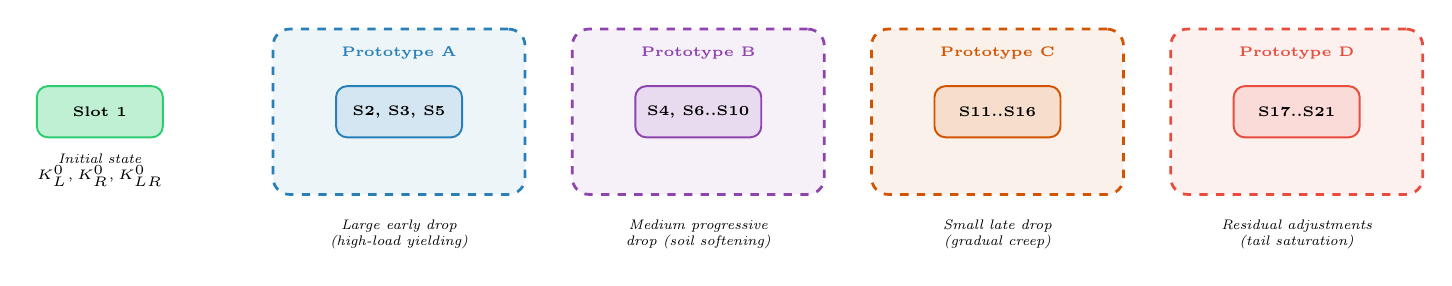
\begin{tikzpicture}[
    >={Stealth[length=2mm]},
    slot/.style={rectangle, rounded corners=4pt, minimum width=1.6cm, minimum height=0.65cm, align=center, font=\tiny\bfseries, draw, line width=0.7pt},
    group/.style={rectangle, rounded corners=6pt, minimum width=3.2cm, minimum height=2.1cm, align=center, draw, line width=1pt, dashed},
]
\node[slot, fill=slotcol!30, draw=slotcol] (s1) at (0, 0) {Slot 1};
\node[font=\tiny\itshape, below=2pt of s1, align=center] {Initial state\\$K_L^0, K_R^0, K_{LR}^0$};

\node[group, fill=teachcol!8, draw=teachcol] (g1) at (3.8, 0) {};
\node[font=\tiny\bfseries, teachcol] at (3.8, 0.75) {Prototype A};
\node[slot, fill=teachcol!20, draw=teachcol] at (3.8, 0) {S2, S3, S5};
\node[font=\tiny\itshape, below=5pt of g1, align=center] {Large early drop\\(high-load yielding)};

\node[group, fill=clustcol!8, draw=clustcol] (g2) at (7.6, 0) {};
\node[font=\tiny\bfseries, clustcol] at (7.6, 0.75) {Prototype B};
\node[slot, fill=clustcol!20, draw=clustcol] at (7.6, 0) {S4, S6..S10};
\node[font=\tiny\itshape, below=5pt of g2, align=center] {Medium progressive\\drop (soil softening)};

\node[group, fill=structcol!8, draw=structcol] (g3) at (11.4, 0) {};
\node[font=\tiny\bfseries, structcol] at (11.4, 0.75) {Prototype C};
\node[slot, fill=structcol!20, draw=structcol] at (11.4, 0) {S11..S16};
\node[font=\tiny\itshape, below=5pt of g3, align=center] {Small late drop\\(gradual creep)};

\node[group, fill=physloss!8, draw=physloss] (g4) at (15.2, 0) {};
\node[font=\tiny\bfseries, physloss] at (15.2, 0.75) {Prototype D};
\node[slot, fill=physloss!20, draw=physloss] at (15.2, 0) {S17..S21};
\node[font=\tiny\itshape, below=5pt of g4, align=center] {Residual adjustments\\(tail saturation)};

\end{tikzpicture}
\end{center}

Then the relation matrix $\mathbf{R}$ would encode rules like:

\begin{itemize}[nosep]
    \item $\mathbf{s}_3 = 0.92 \cdot \mathbf{s}_2$ \quad (Slot 3 is a slightly softer copy of Slot 2)
    \item $\mathbf{s}_5 = \mathbf{s}_2$ \quad (Slot 5 is a reuse of Slot 2)
    \item $\mathbf{s}_7 = 0.75 \cdot \mathbf{s}_4$ \quad (scaled copy within Prototype B)
    \item $\mathbf{s}_{17} = 0.3 \cdot \mathbf{s}_4$ \quad (very small residual from Prototype D)
\end{itemize}

The $\Psi$-M5 student would then use only 5 trainable slot vectors $(1 + 4)$ and reconstruct all 21 slots from $\mathbf{R}$ at every forward pass. If it achieves the same $R^2 = 0.99$ on the test set, we have confirmed that the 21-slot M5 was overparameterized and that the true complexity of the pile stiffness degradation problem requires only 4 independent degradation modes.

\section{Summary}

\begin{table}[H]
\centering
\begin{tabularx}{\textwidth}{@{}lX@{}}
\toprule
\textbf{Aspect} & \textbf{Key Point} \\
\midrule
$\Psi$-NN paper contribution & Automatically discover the best internal structure of a neural network via teacher-student distillation, weight clustering, and structured reconstruction. \\
\addlinespace
M5 role & M5 is already a perfect $\Psi$-NN teacher. It was trained with physics constraints and achieves $R^2 = 0.99$. No modifications needed. \\
\addlinespace
What we discover from M5 & How many truly independent stiffness degradation modes exist in the data; which slots share the same physics; which input features drive which slots. \\
\addlinespace
The $\Psi$-M5 student & A rebuilt model with only $k^*+1$ slot vectors and the discovered structure hardwired via the relation matrix $\mathbf{R}$. Fewer parameters, same accuracy. \\
\addlinespace
Usefulness for pile deformations & Given the predicted $K_L(t), K_R(t), K_{LR}(t)$ sequences, pile-head displacement and rotation under any lateral load history can be computed directly by solving $\mathbf{K}(t) \cdot \mathbf{u} = \mathbf{F}$ at each step. \\
\addlinespace
Scientific value & The discovered slot structure is an AI-learned confirmation (or refinement) of the physical degradation modes assumed in theoretical macroelement models. \\
\bottomrule
\end{tabularx}
\caption{Summary of applying $\Psi$-NN to M5 for pile stiffness degradation.}
\end{table}

\end{document}
